
\documentclass[letterpaper, 10 pt, conference]{ieeeconf}  
\IEEEoverridecommandlockouts                             
\usepackage{graphicx} 
\usepackage{hyperref}
\usepackage{url}

\overrideIEEEmargins

\title{\Huge Target Tracking}
\author{Jiyu Tian} 

\begin{document}

\maketitle
\thispagestyle{empty}
\pagestyle{empty}




%-------------------------------
\section{INTRODUCTION}
The Circulant Matrix (CM) tracker is very efficient finding a translated copy of the target template from the previous frame by computing many convolutions in a single shot. This is accomplished by finding the peak response of a filter applied to a region of the current frame that is expected to include the target. This filter changes from frame to frame and it is computed based on the FFT of a larger region which contains the target in the current frame. Efficiency is obtained by applying this filter in the frequency domain. 



%-------------------------------
\section{ALGORITHMS DESCRIPTION}

\subsection{Basic Algorithm}
The papers describing the algorithm and the code for this tracker is available at:
\url{http://www.robots.ox.ac.uk/~joao/#publications}
and
\url{http://www.robots.ox.ac.uk/~joao/circulant/}.

%-------------------------------
%-------------------------------
\subsection{Detecting Occlusion}
Checking for occlusion can be fulfilled by including a test that measures the response of the filter against the rest of the search window through the use of the ``Peak to Sidelobe Ratio'' (PSR).


The response of the filter is split into the maximum value and the “sidelobe” consisting of the rest of the pixels in the region, excluding a small window (i.e. $11 \times 11$) around the peak. Then the PSR is defined as:
\begin{equation}
    \frac{g_{max} - \mu}{\sigma}
\end{equation}
where $g_{max}$ is the value of the peak, and $\mu$, $\sigma$ are the mean value and the standard deviation of the sidelobe, respectively. A low PSR indicates a poor match and a possible occlusion. If occlusion is detected, the tracker should stop or attempt to hallucinate the target until it can detect it again.





%-------------------------------
%-------------------------------
\subsection{Recovery from Occlusion}
When occlusion is detected, the tracker could use the locations of the target in the past to predict where the target is now (even if it is behind some occluding object) and predict where it should be in the next frame. In this way, rather than giving up, the tracker can attempt to find the target in the next frame at this predicted location. The prediction of the location of the target based on previous measurements can be done using one of many possible methods that we will discuss in class. Among them, the Hankel matrix of the target locations or a simple dynamic model such as constant velocity are taken into consideration.




%-------------------------------
\section{EXPERIMENTAL RESULTS}
We use the \textit{Occluded Face} dataset for this report. In Fig \ref{resp}, while the book crosses in front of the human face, noise is introduced to the response values across image. As the book settles for a couple frames, the noise gradually dies down as the tracker "learns" what the book looks like.


\begin{figure}[thpb]
\centering
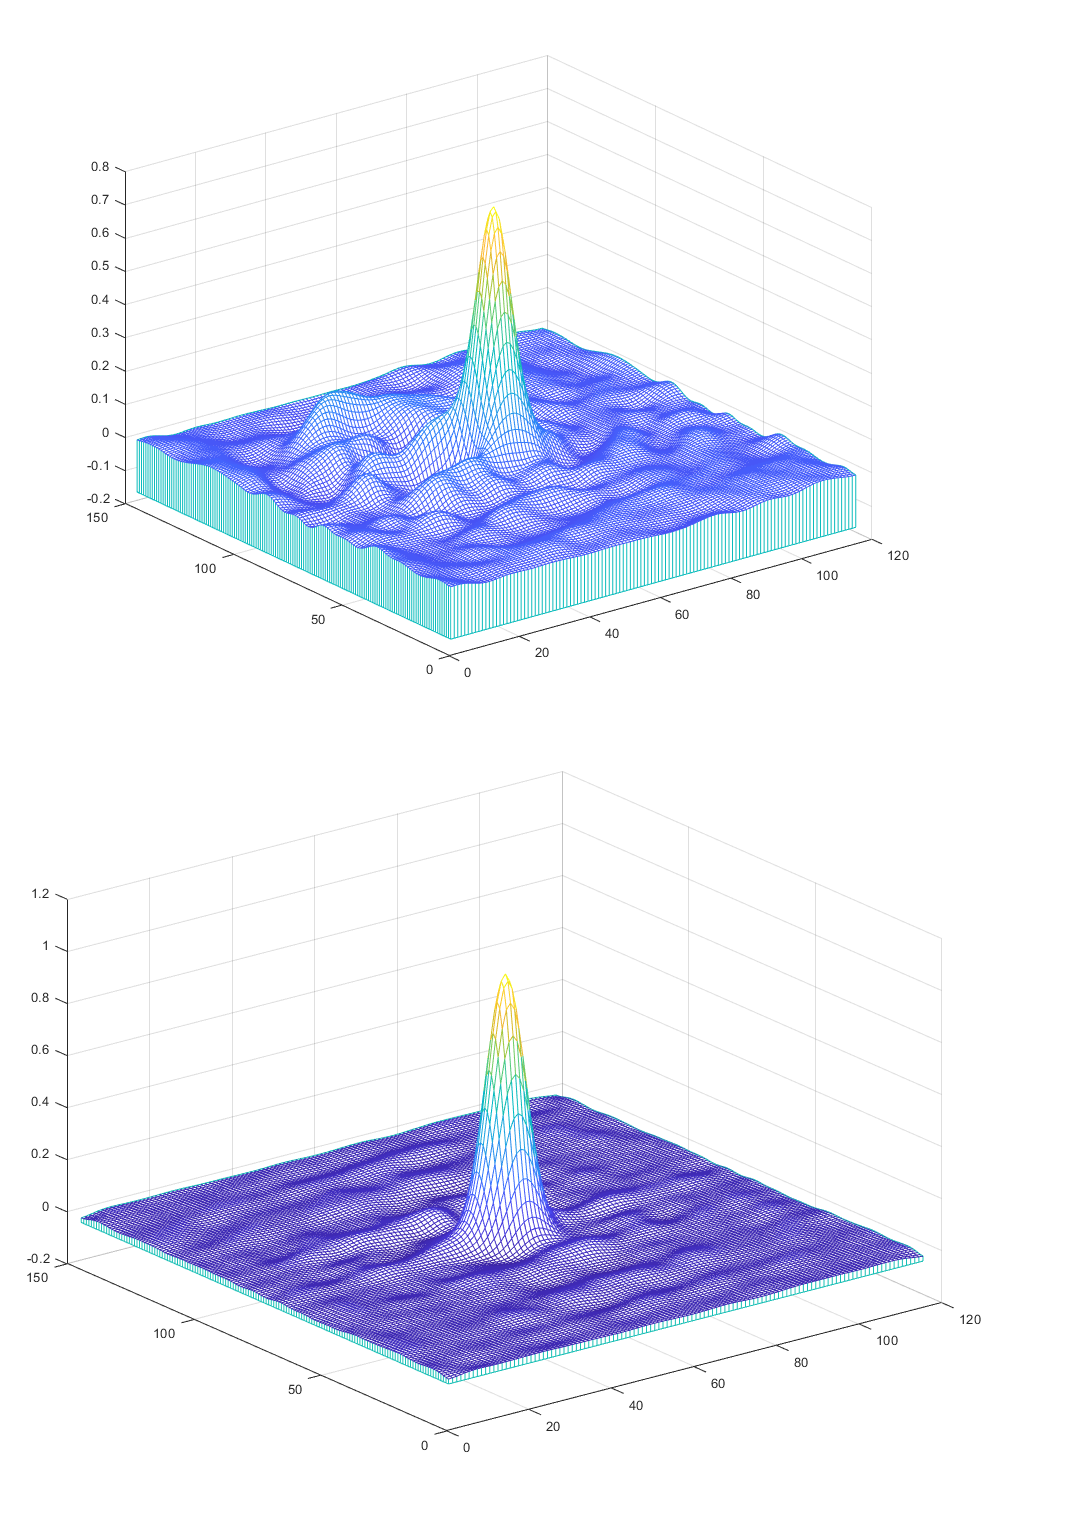
\includegraphics[width=0.5\textwidth]{response.png}
\caption{Response}
\label{resp}
\end{figure}


By computing the PSR, we can estimate how certain the tracker is a particular point represents the center of the tracked object. Low ratio indicates that the tracker is less certain of the outcome with weight being spread across a number of possible pixels. This uncertainty could also represent an occlusion. By thresholding the PSR value, we could estimate when the tracked target was occluded.

As shown in Fig \ref{psr}, whenever the book crosses over the human face, an occlusion is detected. It is always tricky to determine a proper threshold value for detection.


\begin{figure}[thpb]
\centering
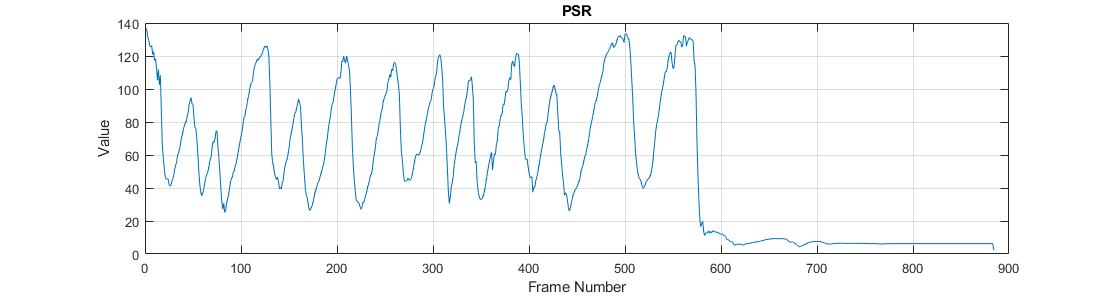
\includegraphics[width=0.5\textwidth]{psr.png}
\caption{PSR}
\label{psr}
\end{figure}

Fig \ref{preg} shows our tracking results (OCC) against the original CM tracker and the original MIL tracker. When threshold is larger than $19$, OCC performs better than CM tracker.


\begin{figure}[thpb]
\centering
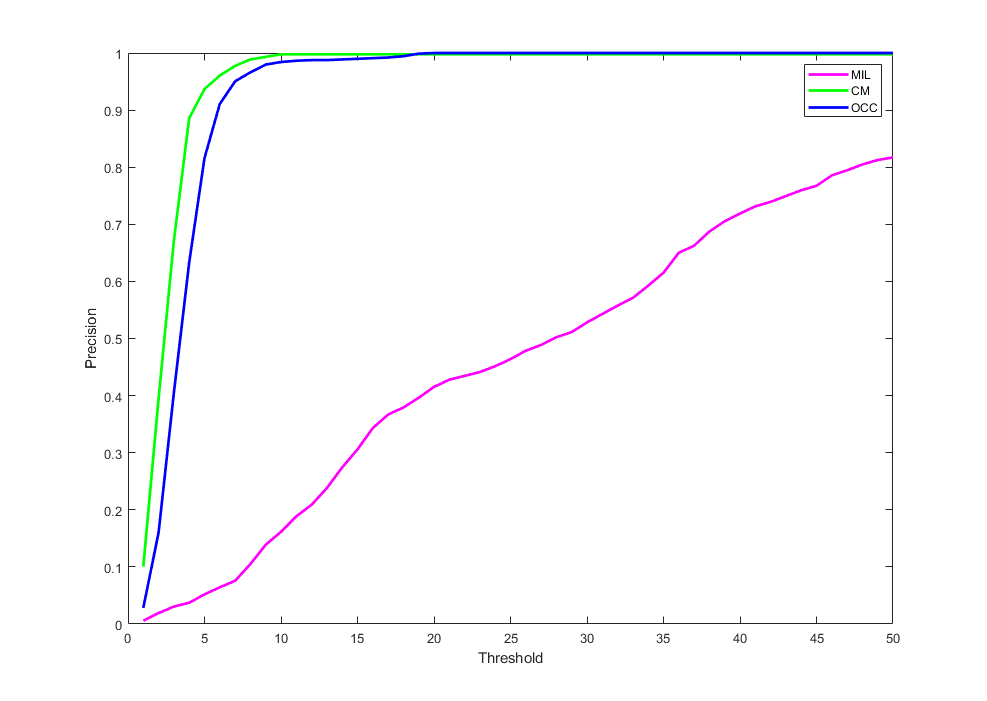
\includegraphics[width=0.48\textwidth]{precisionall.png}
\caption{Precision Graph}
\label{preg}
\end{figure}

Some selections of result figures are shown in Fig \ref{result}.


\newpage


\begin{figure}[thpb]
\centering
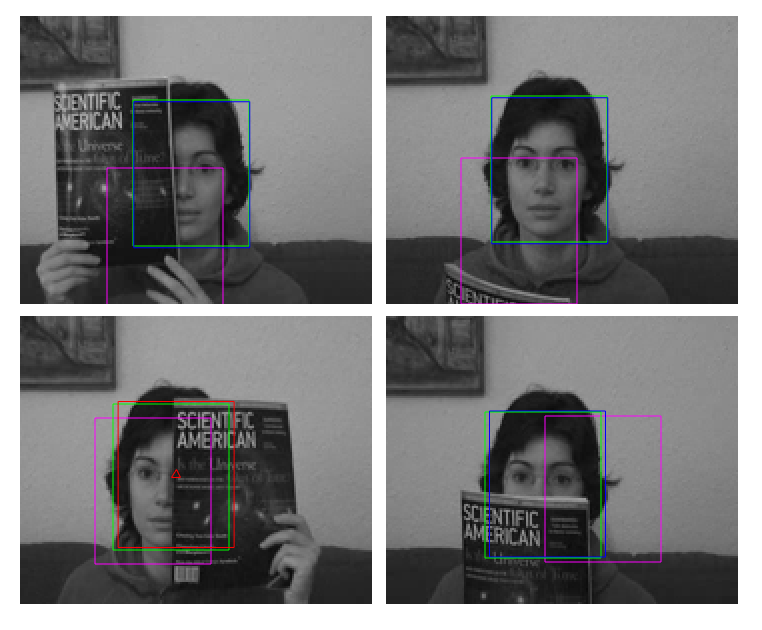
\includegraphics[width=0.491\textwidth]{result.png}
\caption{Precision Graph}
\label{result}
\end{figure}




%-------------------------------
\section{CONCLUSION}
In this project, we improved the CM tracker by implementing an occlusion detection test as well as trying to recover from occlusion. We also explored influence from various parameters, as well as the limitation of the method.




%-------------------------------
\section{Acknowledgements}
The original Circulant Matrix Tracker from the following paper: \textit{Henriques, Joao F., et al. "Exploiting the circulant structure of tracking-by-detection with kernels." European conference on computer vision. Springer, Berlin, Heidelberg, 2012.}


\end{document}
